% !TEX program = xelatex
% !TEX encoding = UTF-8
\ifcsname wholebook\endcsname
\else
\documentclass[12pt,a4paper]{ctexbook}
% ============================================================
% 共享导言区 preamble.tex
% 本文件被 main.tex(整书编译)和各章文件(单独编译)共同引用,
% 从而保证两种编译方式下的宏包与样式完全一致。
% 注意: 本文件不含 \documentclass, 只放宏包与样式设置。
% ============================================================
\usepackage[a4paper,margin=1.1in]{geometry}
\usepackage{graphicx}
\usepackage{listings}
\usepackage{xcolor}
\usepackage[hidelinks]{hyperref}
\usepackage{tikz}
\usetikzlibrary{positioning,arrows.meta,decorations.pathreplacing,calc}
\usepackage{booktabs}

% 代码环境样式设置
\lstset{
    basicstyle=\ttfamily\small,
    keywordstyle=\color{blue}\ttfamily,
    commentstyle=\color{gray}\ttfamily,
    stringstyle=\color{red}\ttfamily,
    backgroundcolor=\color{gray!8},
    frame=single,
    rulecolor=\color{gray!40},
    breaklines=true,
    showstringspaces=false,
    columns=fullflexible,
    keepspaces=true,
    % 允许中文注释/内容正常显示
    extendedchars=true,
    literate={
        {·}{{\cdot}}1
    }
}

\begin{document}
\fi

\chapter{Ubuntu环境下编程}
做机器人最常用的两门语言就是C++和Python，同时这两门语言也是编程语言流行度排行榜数一数二的。然后这两门咱们都学过。C++是课上教的，python语法极其简单，不赘述了。

一般用Linux的都是程序员里的大佬，都是大佬了，一般就喜欢拿记事本grdit写代码，因为不用打开编辑器，全程可以在命令行终端里执行。Linux里面还有逆天Vim，但此等极道帝兵显然不是我等炼气期小辈能够掌握的。以后编程估计都在VS code里完成，但是先看一下Ubantu里面程序的运行和编写和Windows下有何不同。
\section{Hello weijianguizhou！}
\subsection{C++}
打开终端，创建一个d2lros2文件夹接着在文件夹下创建chapt1文件夹。
然后输入这行命令：
\begin{lstlisting}[language=bash,title={用gedit创建并打开cpp文件}]
    gedit hello_weijianguizhou.cpp
\end{lstlisting}
输入：
\begin{lstlisting}[language=c++,title={cpp程序}]
    # include <iostream>
    using namespace std;
    int main(){
    	cout<<"Hello weijianguizhou!"<<endl;
    	return 0;
    }
\end{lstlisting}
保存代码，关闭gedit。

C++代码必须经过编译构建之后才能运行

C++的编译工具使用的是g++，默认是不安装的，所以我们需要手动安装一下g++。
\begin{lstlisting}[language=bash,title={安装g++编译器}]
    sudo apt install g++
\end{lstlisting}
接着在终端输入下面的指令对刚刚的代码进行编译。
\begin{lstlisting}[language=bash,title={编译C++}]
    g++ hello_weijianguizhou.cpp
\end{lstlisting}
接着使用ls指令，应该可以看到一个叫做a.out的文件。恭喜，现在可以运行了。
\begin{lstlisting}[language=bash,title={运行C++}]
    ./a.out
\end{lstlisting}
可以看出区别了。Windows系统中的可执行文件为.exe，而Linux系统中的可执行文件为.out.

真尼玛麻烦。

\subsection{python}
然后输入这行命令：
\begin{lstlisting}[language=bash,title={用gedit创建并打开py文件}]
    gedit hello_weijianguizhou.py
\end{lstlisting}
输入
\begin{lstlisting}[language=python,title={py程序}]
print("Hello weijianguizhou!")
\end{lstlisting}
保存代码，关闭gedit。
直接运行：
\begin{lstlisting}[language=bash,title={运行py}]
    python3 hello_weijianguizhou.py
\end{lstlisting}

下面看一下python和C++对比。
\begin{figure}[htbp]
  \centering
  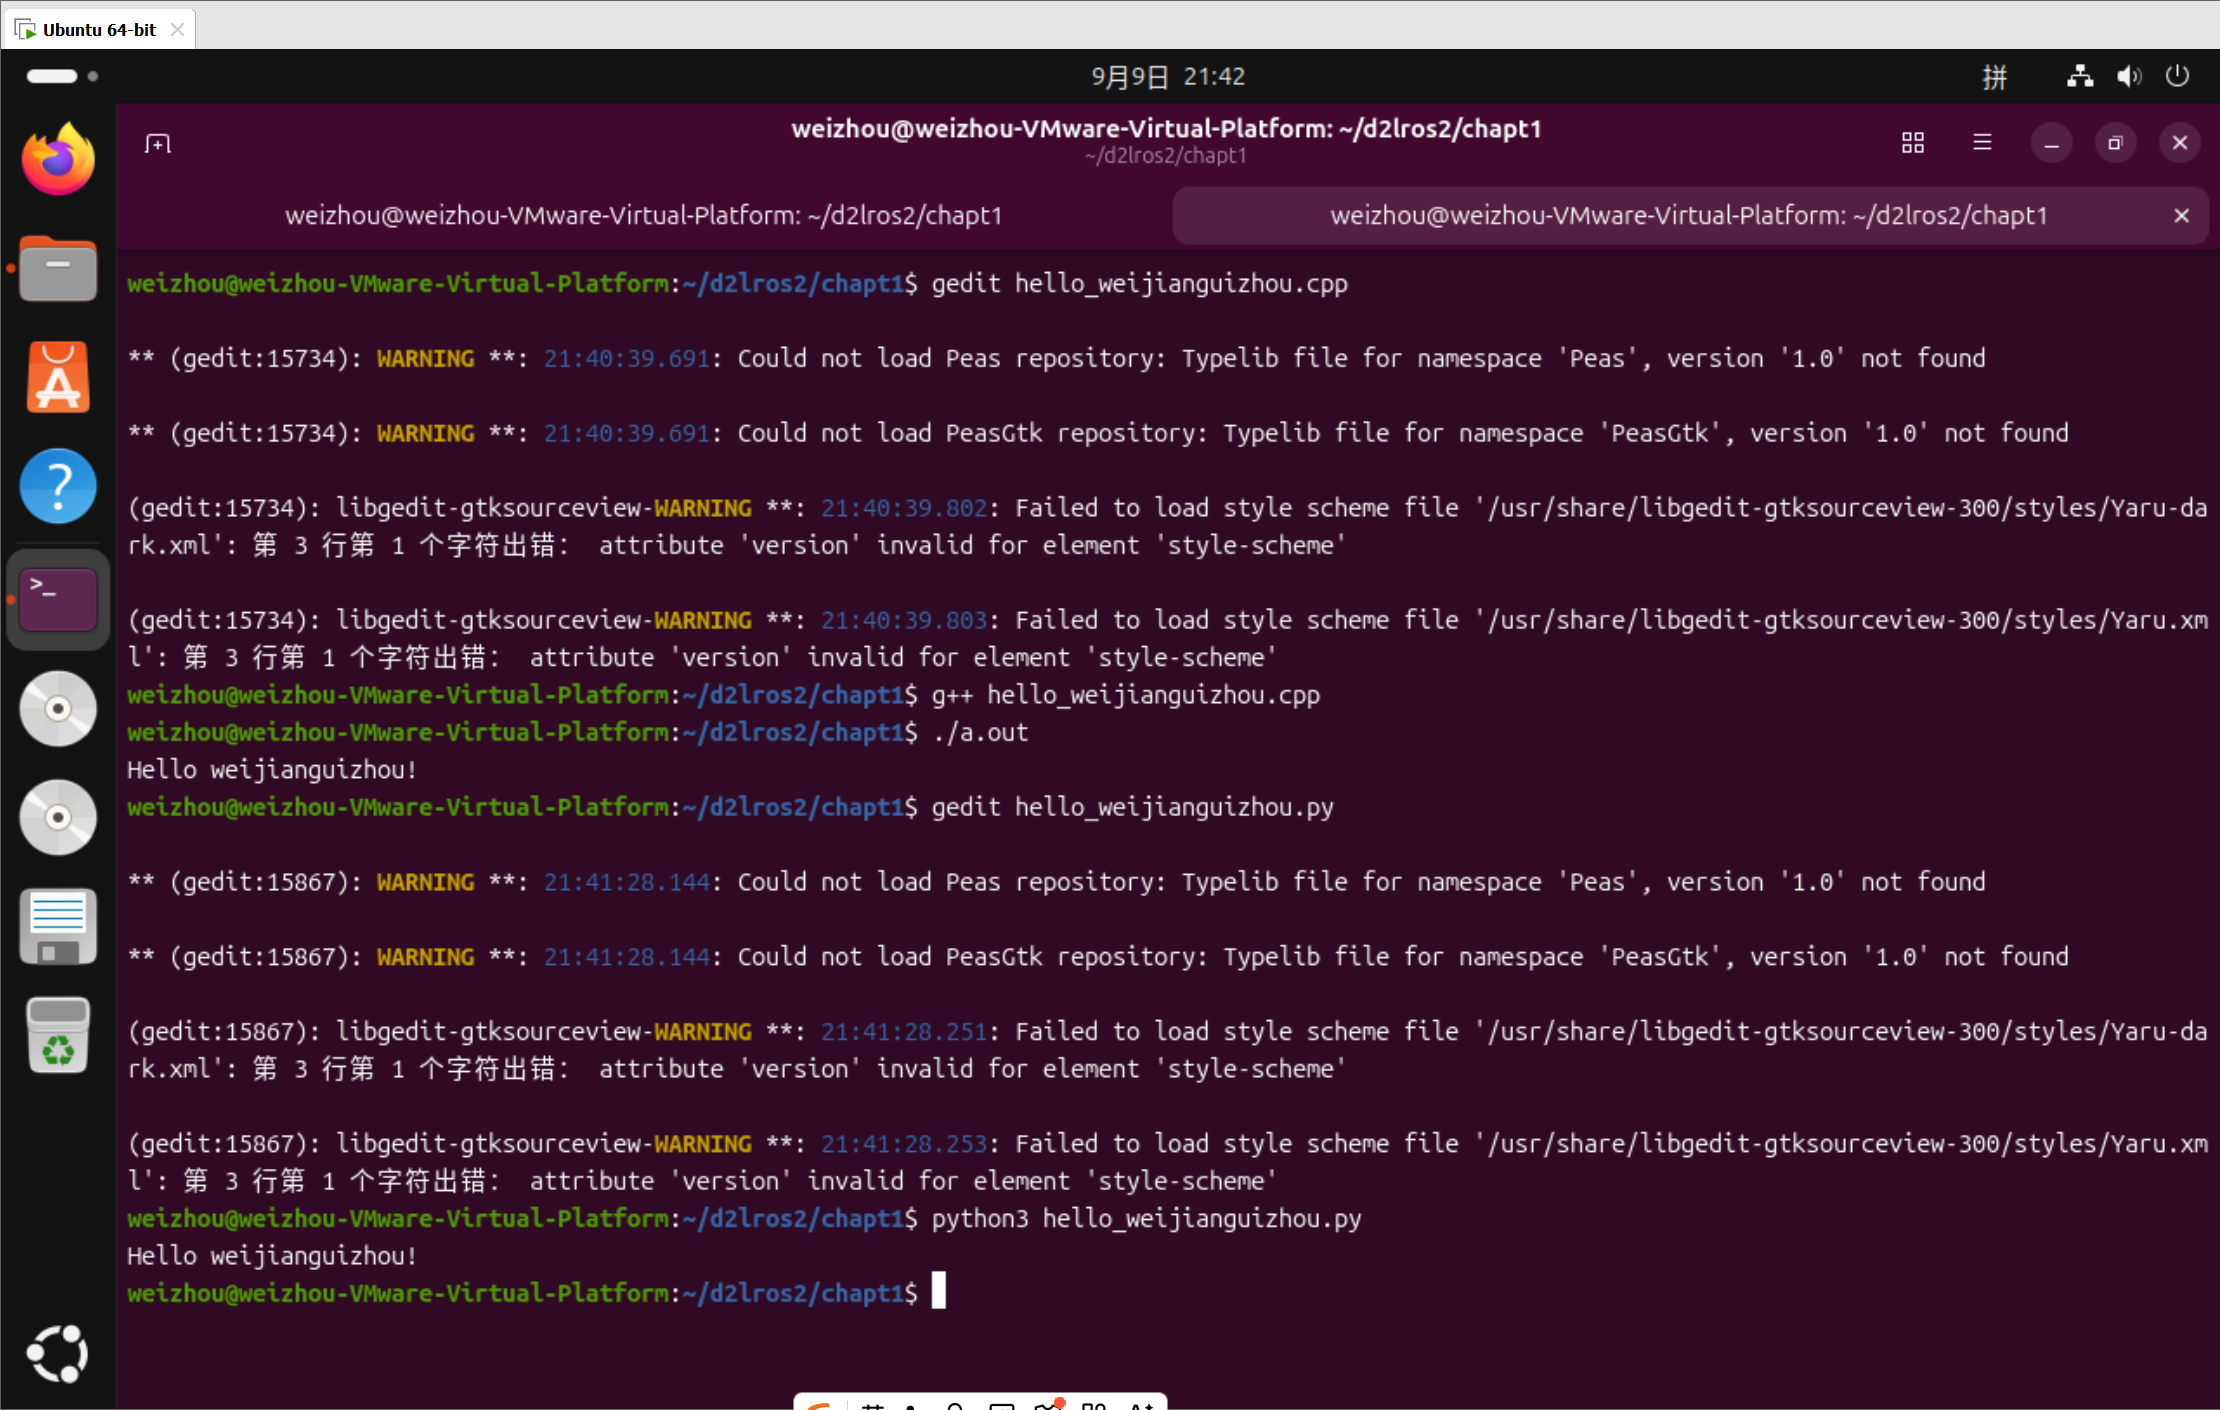
\includegraphics[width=0.8\textwidth]{Figure/python和C++对比.png}
  \caption{python和C++对比}
  \label{fig:python和C++对比}
\end{figure}
由此看来，python相比C++有如下优势：

一、python程序比C++简单。C++要6行才能搞定的程序我python只要1行就能搞定，此乃一胜。

二、python在命令行中的运行比C++简单。C++最短要三行，而我python只要一行，此乃二胜。

三、python语法更接近自然语言。此乃三胜。

由此看来，python大获全胜......吗？？？

并非啊！虽然python好用，但是它，慢啊！！！

为啥？

因为C++ 是编译执行，而python是解释执行。

\section{什么是编译执行和解释执行}
语言本身用解释型语言还是编译型语言来划分就是不准确的。

设计语言的人，也不会考虑先考虑什么型，而是在设计中发现某种方式更好，便会选择使用。语言属于XX型是呈现给大家的一个印象。

编程语言，是程序员们操控电脑以实现各种功能的主要方式，而解释执行与编译执行，是计算机编程语言的两种执行方式。

更多的时候，某个语言使用到了编译执行也用到了解释执行。

现在来笼统解释一下。
\begin{itemize}
    \item 编译：将源代码一次性转换为机器码的过程（机器码有保存为文件，下次运行的时候直接运行机器码）
    \item 解释：将源代逐行转换为机器码并运行的过程（机器码并没有保存下来）
    \item 编译执行（编译器）：将一段程序直接翻译成机器码(对于C/C++这种非跨平台的语言)或者中间码(Java这种跨平台语言，需要JVM再将字节码编译成机器码)。编译执行是直接将所有语句都编译成了机器语言，并且保存成可执行的机器码。执行的时候，是直接进行执行机器语言，不需要再进行解释/编译。
    \item 解释执行（解释器）：在执行程序时，再将中间码（例如Java的字节码通过JVM解释成机器码）一行行的解释成机器码进行执行。这个运行过程是解释一行，执行一行。
\end{itemize}

执行编译过程的程序叫做编译器。

执行解释过程的程序叫做解释器。

王垠所说的编译型语言和解释型语言的本质都是解释执行的。

编译型和解释型的语言之所以可以说相同，是因为这些语言从文本形式的源代码到最终产生的结果，所经历的过程是一样的。

根本区别是运行时，解释型需要将程序解释成机器码来运行，并没有保存机器码，是在运行过程中进行。

而编译型在运行之前就已经让编译器给程序编译成机器码了。

这也是为什么编译运行会比解释运行快的根本原因。

在知乎上看到一个比喻，非常好。

编译相当于做好了一桌子菜，可以直接开吃了。

而解释就相当于吃火锅，需要一边煮一边吃。

那么自然，吃的效率也会低一些。


\ifcsname wholebook\endcsname
\expandafter\endinput
\fi

% 单独编译模式: 在顶层(无未闭合条件)执行 \end{document} 收尾。
\end{document}